\documentclass[11pt]{article}
\usepackage{hyperref}
\usepackage[english]{babel}
\usepackage{blindtext}
\usepackage{url}
\usepackage{graphicx}
\usepackage{multicol}
\usepackage{geometry}
\usepackage[sort, numbers]{natbib}

\usepackage [autostyle, english = american]{csquotes}
\MakeOuterQuote{"}

\usepackage{fancyhdr}


\graphicspath{ {/home/joebrew/Documents/uf/phc6016/loi} }


\usepackage{Sweave}
\begin{document}
\Sconcordance{concordance:loi.tex:loi.Rnw:%
1 20 1 1 0 84 1 1 43 1 2 4 1 1 13 1 2 10 1}


\newgeometry{margin=1.5cm}
\fancyhfoffset[E,O]{0pt}

%------------------------------------------
\section*{Childhood obesity in a diverse school-aged population: place, race and time}
%------------------------------------------
Joe Brew | Dept. of Epidemiology | University of Florida | joebrew@gmail.com | 352.318.4553 | databrew.github.io

\noindent \hrulefill

\vspace{5mm}
\noindent Dear Sir / Madam,

Thank you for your consideration of my proposal, "Childhood obesity in a diverse school-aged population: place, race and time".  I believe that this project fits well into the Robert Wood Johnson Foundation's focus on inequalities in childhood obesity, and has the potential to guide policy which will help children "to lead the healthiest lives they can."  


%------------------------------------------
\subsection*{Introduction}
%------------------------------------------
The prevalence of obesity among American school-aged children has grown in recent decades at an alarming rate (figure 1)\cite{Ogden2014}. Obesity has a steep social gradient, and areas that are poor or socially marginalized have above average rates in the USA.\cite{Budd2014} Because obesity is closely correlated with socieconomic status, which is in turn associated with residential location, studying geography's independent association with childhood obesity is a methodological challenge. 

Alachua County, Florida, offers the ideal location to confront this challenge (figure 2).  The Alachua County Public Schools system\cite{acps} collects a wealth of data on the health of its more than 30,000 students, and maintains databases with reliable information going back over a decade.  Furthermore, Gainesville (Alachua's largest city) has recently established an "open data portal," allowing for quick and easy access to information on public safety, infrastructure/transportation, and government spending.\cite{gnv}  The combination of these two datasets allows for the discovery of child adiposity's strongest associations; and the historical element faciliates exploration of obesity's causal dimensions.

Alachua is a diverse county both geographically (rural/urban) and racially (46\% of Alachua public school students are non-white)\cite{Brew2014}.  Socioeconomically, Alachua's 41 public schools include multiple highly-ranked magent programs, which has the effect of attracting students from families who might otherwise send their child to a private institution.

Though numerous explanations have been offered for the steep increase in the \emph{prevalence} of childhood obesity in recent decades\cite{Bishop2005}, and health inequalities in childhood obesity have been explored at the macro level\cite{2013}\cite{Drewnowski2009}, little is known about what affects childhood obesity \emph{within} a community. This study proposes to examine those factors with the hope of elucidating causal pathways to childhood obesity, and in doing so, inform community-level interventions. 

%------------------------------------------
\subsection*{Aims}
%------------------------------------------
The primary purpose of this project is to assess and quantify variance in childhood obesity.  Questions to be addressed include:
\begin{enumerate}
\item Which social, economic, demographic and geographic features are most closely associated with childhood obesity?
\item What role does residential environment (neighborhood) play in the development of childhood obesity over time, after adjustment for relevant social confounders?
\item Of childhood obesity's causal factors, which are "modifiable" at the community-level, and how confident can policy-makers be that "built environment" interventions will have their intended effect?
\end{enumerate}

%------------------------------------------
\subsection*{Statement of need}
%------------------------------------------
Among Alachua County schoolchildren, the obesity rate is 18.14\% and the overweight rate is 37.74\%. Additionally, inequality in obesity is high: the prevalence of obesity is highest among black (22.08\%) and multiracial (26.67\%) students, and students who qualify for free/reduced lunch are 67\% more likely to be obese than those who don't.\cite{Brew2014}    

Assessing the causes of childhood obesity at the community level is urgent for two reasons.  First, the lack of research in the area leaves community and public health practitioners with little ground to stand on when it comes to "best practice" in non-clinical and population-level interventions.  Second, given that even the most ambitious (and least realistic) federal governments policy changes are unlikely to seriously reduce the prevalence of childhood obesity in the next 20 years\cite{Kristensen2014}, it is crucial that communities 

%------------------------------------------
\subsection*{Methodology}
%------------------------------------------
This project consists entirely of secondary data collection and analysis.  Student data will consist of health screening records (age, weight and height in first, third, sixth and ninth grade), residential location, free/reduced lunch status, and race/ethnicity.  Neighborhood features will be constructed using a combination of aggregated student data (e.g. characteristics of nearest peer neighbors), as well as data from the Gainesville open data portal and the United States census.  Feautres to be constructed include infrastructure ammenities (distance to nearest park, percent of fastest route to school with bike lanes and/or sidewalks), food options (ratio of grocery to convenience stores), crime rate, and economic growth (rate of new business opening and new home constructions per 1,000 residents).  "Neigbhorhoods" will be defined as census blocks. Analysis will be iterative, but will have three main phases.
\begin{enumerate}
\item Exclusive analysis of outcome (BMI percentile for age) by geography using Kulldorff's method for detecting "clusters" or "hotspots".\cite{Kulldorff1997} Though more commonly used for the identification of communicable disease and other non-chronic condition outbreaks, the Kulldorff scan statistic will be useful in identifying areas where children are much more likely to be obese; this, in turn, will inform how model features should be constructed in the second phase.
\item Feature construction, using qualitative insights gained in phase 1, will be the most laborious phase. Neighbhorhood characteristics will be compiled into multiple indexes (such as walkability, community cohesiveness, urban/rural-ness, safety, marginalization, etc.), each with multiple variations. In addition to community-level feature construction, student-level data will also be engineered so as to reflect changes over time (e.g. a student coming off free lunch or changing residences). Though a surplus of predictors might be problematic using traditional methodology, the "machine learning" component of the anlaysis in the third phase means that a multitude of similar predictors will be advantageous to fitting a model. 
\item Random forest classification will be used to model adiposity outcomes.  Random forest methodology (as opposed to traditional linear / frecuentist statistics) is preferred in that its use of bootstrap aggregation ("bagging") allows for better predictor selection as well as the ranking of predictor importance.
\end{enumerate}

The model will be "trained" on data from the 2003-2004 to 2013-2014 school years and validated on data from the 2014-2015 school year.  Geospatial mapping of model misprediction will inform where the model is strongest and weakest, and allow for posterior predictor adjustment, if applicable.  

%------------------------------------------
\subsection*{Conclusion}
%------------------------------------------

We live in a time of a rapid increase in childhood obesity, a plethora of new and innovative computing methods, and a wealth of data.  Through the use of the latter two, this project aims to address the former.    
The results of this study, both in terms of the methods used as well as the correlations uncovered, will inform both further research as well as community-level policy and practice.  

\vspace{3mm}

\noindent Thank you for your consideration.  Please do not hesitate to contact me if you have any questions.
\vspace{5mm}

\noindent Joe Brew

%----------------------------------------------------------------------------------------
\subsection*{Figures}
%----------------------------------------------------------------------------------------
\begin{center}
Figure 1: Obesity among American children\cite{NIH}
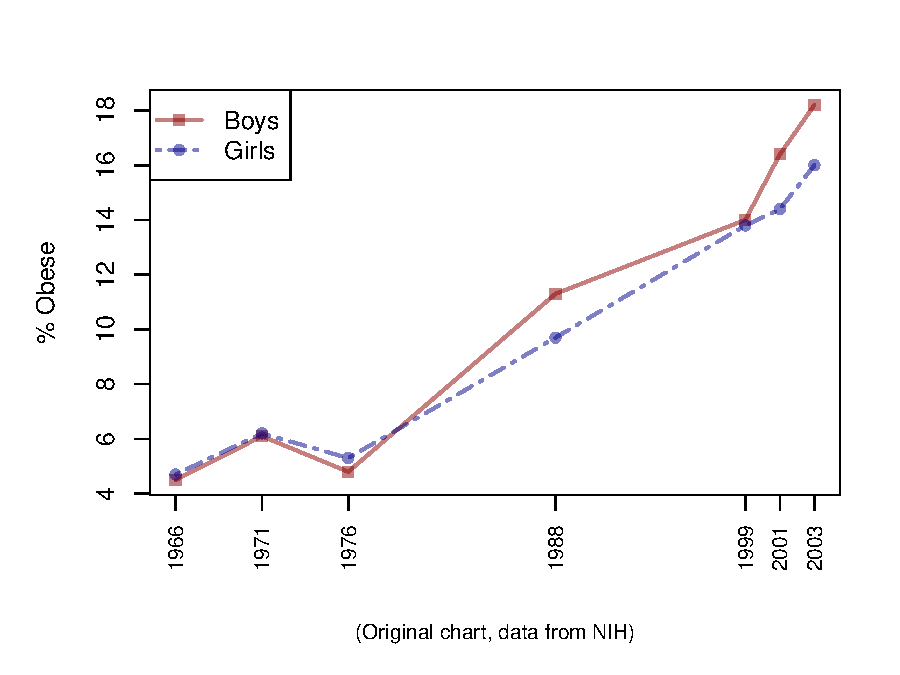
\includegraphics{loi-001}
\end{center}


\begin{center}
Figure 2: Alachua County, Florida\cite{maps}
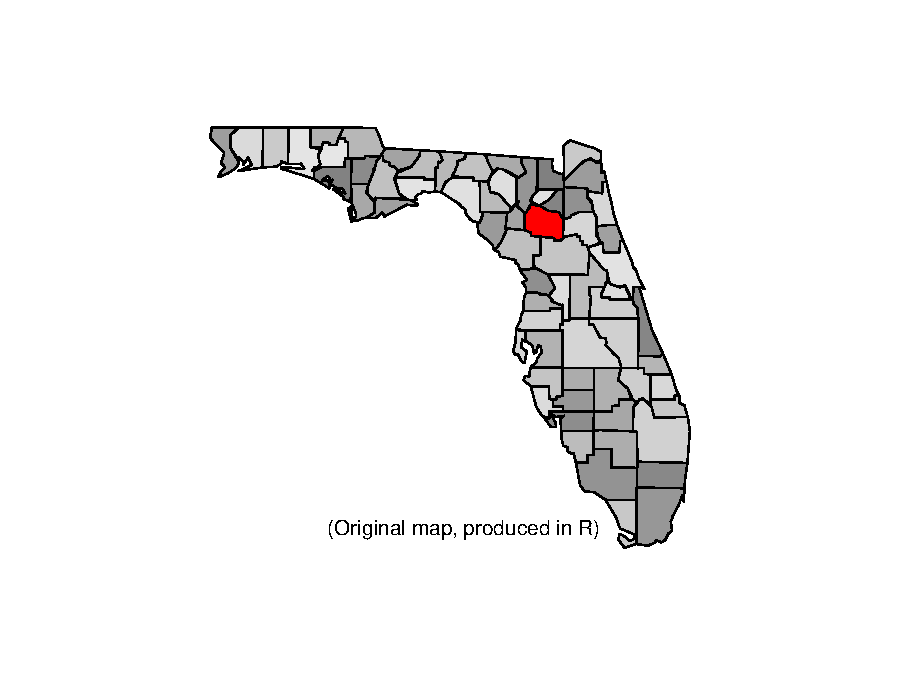
\includegraphics{loi-002}
\end{center}
%----------------------------------------------------------------------------------------
%  REFERENCE LIST
%----------------------------------------------------------------------------------------
\bibliographystyle{unsrtnat}
\bibliography{test}




\end{document}
